\documentclass[11pt,onecolumn]{article}
\usepackage{makeidx,times,alltt,graphicx,calc,subfigure}
\usepackage{epstopdf}
\usepackage{xspace}
\usepackage{longtable}
\usepackage{wrapfig}
\usepackage{fancyvrb}
\usepackage{booktabs}
\usepackage{ctable}
\usepackage{multirow}
\usepackage{bigdelim}
\usepackage{ctable}
\usepackage{graphicx}
\usepackage{subfigure}
\usepackage{fancyvrb}
\usepackage{color}
\usepackage{listings}
\usepackage{epsfig,alltt}
\usepackage{graphics}
\usepackage{shortvrb}
%\usepackage[english,ruled,vlined]{algorithm2e}
%\usepackage{latexsym}
%\usepackage{amssymb,amsmath}
%\usepackage[usenames]{color}
\usepackage{setspace}
\usepackage{comment}
%\usepackage{ulem}

\usepackage{listings}
\lstset{fancyvrb=true}
\lstset{
    language=C++,
        basicstyle=\footnotesize\tt,
        %basicstyle=\tt, 
        %keywordstyle=\color{blue},
        identifierstyle=,
        %commentstyle=\color{green},
        %stringstyle=\color{red},
        showstringspaces=false,
        captionpos=t,
        tabsize=3,
        %linewidth=12mm,
        numbers=left, 
        stepnumber=2
}

%\usepackage{pdftricks}
%\begin{psinputs}
%\usepackage{pstricks}
%\usepackage{color}
%\usepackage{pstcol}
%\usepackage{pst-plot}
%\usepackage{pst-tree}
%\usepackage{pst-eps}
%\usepackage{multido}
%\usepackage{pst-node}
%\usepackage{pst-eps}
%\end{psinputs}

%\newcommand{\comment}[1]{}
\newcommand{\charmpp}{\textsc{Charm++}}
\newcommand{\namd}{\textsc{namd}}
\newcommand{\charisma}{Charisma}
\newcommand{\divcon}{\emph{DivCon}}
\newcommand{\openatom}{\textsc{OpenAtom}}
\newcommand{\LeanCP}{\textsc{OpenAtom}}
\newcommand{\leancp}{\textsc{OpenAtom}}
\newcommand{\changa}{ChaNGa}
\newcommand{\kale}{Kale}
\newcommand{\sdag}{Structured Dagger}
\newcommand{\parfum}{{\sc ParFUM}}
\newcommand{\metis}{{\sc Metis}}
\newcommand{\note}[1]{\emph{(Note: #1)}}
\newcommand{\tight}{\baselineskip=8pt}
\newcommand{\etal}{{\em et al.}}
\newcommand{\viz}{{\em viz.}}
\newcommand{\nbody}{$N$-body}
\newcommand{\kdtree}{$k$d-tree}

\def\code#1{{\small {\tt {#1}}}}
\def\smallfbox#1{{\small {\fbox{#1}}}}
\def\porder#1#2#3{$#1 <_{#3} #2$}
\def\lhs#1#2{$#2 \in \mathit{LHS}(#1)$}
\def\rhs#1#2{$#2 \in \mathit{RHS}(#1)$}


\oddsidemargin=-0.25in
\textwidth=7in
\topmargin=-0.25in
\headheight=0in
\headsep=0in
\textheight=9.5in

\begin{document}
%\doublespacing

\title{ ECE598KH Final Project Report \\ NAMD GPU Performance Analysis and Tuning}

\author{
  Yanhua Sun, Xin Zhao\\
  University of Illinois at Urbana-Champaign\\
  \{sun51, xinzhao3\}@illinois.edu
}

\date{}
\maketitle

\lstset{
  basicstyle=\ttfamily,
  showstringspaces=false
}

%\begin{tight}
%\bibliographystyle{abbrv}
%\bibliography{group,cited}
%\end{tight}

\section{Introduction}
In this project, the application we are focusing on is NAMD.
NAMD~\cite{NamdSC02}, recipient of a 2002 Gordon Bell Award, is a parallel molecular 
dynamics code designed for high-performance simulation of large biomolecular systems.
It was developed in the mid-1990's. Now it is one of the most widely used molecular dynamics 
software with more than 50,000 users. It was also selected by NSF as an acceptance test
for Blue Waters.
Through many years, NAMD has been highly optimized to achieve scalable performance on CPU.
It has successfully scaled to the full Titan supercomputer with around $300K$ cores and 
the full Blue Waters with $400K$ cores.

These years, GPU-accelerated algorithms have demostrated speedup of 10- to 100-fold. Meanwhile, 
the hardware has been improved significantly to better match the needs of algorithms over the years.
Since 2006, NAMD has been accommodated to take the advantage of GPU-accelerators. Speedup of 
6- or even 10- has been demonstrated in the previous work~\cite{phillips_stone_namd_cuda}.
Although NAMD GPU has been carefully designed and optimized, it still needs a lot of 
efforts to maximize the performance on GPU, especially on the new hardware such as Fermi, Kepler. 

In this report, we first analyzed NAMD performance on two machines with different configurations.
One is with fast CPU but slow old GPU while the other has fast CPU but slower CPU. We showed 
the results and explained the reasons. Based on our analysis, we optimized the GPU kernel code
to reduce the GPU time. This optimization helps when GPU becomes performance bottleneck.
At the same time, due to the difference of total CPU and GPU capabilities, the load between them
can be imbalanced. We also proposed and implemented a load balancing strategy between CPU and GPU.
We demostrate the effectiveness of our optimizations by comparing the original performance results
and new results.

%\namd{}

\section{NAMD GPU Design } 
\textbf{Parallel Design}: Figure~\ref{figs:parallelmd} illustrates the design of NAMD decomposition.
The parallel structure of NAMD is based on a unique object-based
hybrid decomposition, parallelized using the \charmpp{} programming model.
Atomic data is decomposed into spatial domains (called ``patches''
shown in yellow box in figure) based on the short-range
interaction cutoff distance such that in each dimension only atoms in
one-away or, when necessary to increase concurrency, one-away and two-away
neighboring domains will interact directly.
These equally-sized domains are distributed as evenly as possible across
the machine and are responsible for accumulating forces and integrating
the equations of motion asynchronously via per-domain user-level threads.
Patches are represented on other cores by proxies and all position
and force data sent between cores passes via these proxy patches.

The calculation of short-range interactions is orthogonally decomposed
into ``compute objects'' (shown in red diamond) representing interactions between atoms within
a single domain, between pairs of domains, or for groups of neighboring
domains for terms representing multi-body covalent bonds.
Compute objects are scheduled by local prioritized \charmpp{} messages
when updated position data is received for all required patches.
Longer-running domains are further subdivided by partitioning their outer
interaction loops to achieve a grain-size that enables both load balancing
and interleaving of high-priority PME or remote-atom work with
lower-priority work that does not require off-node communication.

\begin{figure}[h]
\centering
\includegraphics[width=2.8in]{figs/parallelmd}
\caption{NAMD decomposition}
\label{figs:parallelmd}
\vspace{-0.2cm}
\end{figure}

\textbf{GPU and CPU work assignment}:
NAMD offloads only short-range non-bonded calculations to the GPU
as these are the most expensive part of the calculation, are best suited
to the GPU architecture, and do not require additional communication stages.
Every non-bonded compute object assigned to a given GPU is mapped to one or
two GPU multiprocessor work units (``blocks'' in CUDA).
Although GPUs support very fine-grained parallel decomposition internally,
the interface presented to the controlling CPU requires data and work to
be aggregated for efficiency.
When all required position data is received on the CPU, it is then copied
to the GPU and two sets of work units are scheduled.
The first set calculates forces for remote atoms, which require off-node
communication, and the second set calculates only forces for local atoms.
This allows some overlap of communication and computation~\cite{phillips_stone_namd_cuda}.





\section{NAMD GPU CPU Load Balance}
\label{sec:balance}
As we described earlier, in \namd{} GPU design all nonbonded work 
is offloaded to GPU since its computation is most intensive.
In code shown in ~\ref{gpu-cpu-assignment}, it is implemented by assigning computes to GPU so long as 
it has the types of Nonbonded*, which include NonbondedPair and
NonbondedSelf.  

%\begin{lstlisting}[float,frame=single,caption={Compute Assignment},label=gpu-cpu-assignment]
\begin{lstlisting}[frame=single,caption={Compute Assignment},label=gpu-cpu-assignment]
switch ( type of compute )    
{
    case computeNonbondedSelfType:
            register_cuda_compute_self(i,map->computeData[i].pids[0].pid);
            break;
    case computeNonbondedPairType:
            register_cuda_compute_pair(i,pid2,trans2);
            break
   ........................
   other types:
            create computes on CPU
            break;
}

\end{lstlisting}

\textbf{Motivation} : While this is a straightforward way to balance load between CPU and GPU, 
it may have significant performance problem depending on the configuration
of GPU and CPU.

Figure~\ref{figs:gpu-ppn1} and ~\ref{figs:gpu-ppn15} show the timeline of 
running $92,224$ atom Apoa1 using 1 GPU and 1 CPU core, 1GPU and 15 CPU cores.
Each main line represents execution on one CPU core. Different colors stand for 
different function execution. The red activity is for integration while the purple
is all bonded work on CPU. The white color stands for idle time. The green bars on top of the main bars 
show the execution of GPU. In Figure~\ref{figs:gpu-ppn1}, the total time range 
is around $117 ms$, which is the time for one simulation step. We can see that
GPU only takes a small portion of total time, which is around $19 ms$.
In this case, it is correct that we should offload as much nonboned work as possible
to GPU since CPU execution is relatively slow. 

However, in Figure~\ref{figs:gpu-ppn15} when we increase the number of CPU cores, 
the work on CPU side is parallelized and time is reduced to $12 ms $ while the GPU exection
still takes $19 ms$. As a result, on CPU side, there is a big portion of idle time.    

\begin{figure}[h]
\centering
\subfigure[1CPU core + 1 GPU] {\label{figs:gpu-ppn1}\includegraphics[width=5.8in]{figs/gpu-ppn1-timeline-117ms.png}}
\subfigure[15 CPU cores + 1 GPU] {\label{figs:gpu-ppn15}\includegraphics[width=5.8in]{figs/gpu-ppn15-timeline-117-25ms.png}}
\caption{Timeline of running Apoa1 with 1 GPU and different number of CPU cores}
\label{figs:cpu-gpu}
\end{figure}



%\section{Background}
%In a molecular dynamics simulation, a collection of atoms interact through a set of forces. 
%Since each atom interacts with all the other atoms, the complexity of calculating forces
%is $O(Atoms^2)$. This algorithm does not scale with the number of atoms. Based on the fact that
%atoms from far distance contribute little to the force calculation, in \namd{} the interaction is
%calculated by short range forces and long range forces. The molecule  is spatially divided into 
%patches based on cutoff distance. Atoms in one patch only interact with other atoms in neighbor patches.
%To be more accurate, long range electrostatics calculation is performed through particle-mesh Ewald (PME) method.
%For these two types of calculation, short range forces are computation intensive while PME is communication intensive.
%Therefore, in current NAMD GPU design and implementation, non-bonded cutoff computation is offload to GPU.
%All other bonded work, integration and PME work is remained on CPU.

%\section{Objective}

\section{NAMD GPU Kernel Optimization}
\subsection{GPU Force Calculation Kernel}

In the original GPU kernel implementation, each thread block calculates the forces on the atoms in one patch (patch 1)
due to the atoms in another patch (patch 2). Fig.~\ref{figs:pseudocode} presents the pseudo-code for kernel calculation.
In the outer loop, each thread copies atoms from patch 1 to local registers. In the inner loop. threads in the block collaborate to
load atoms from patch 2 to shared memory. Before and after reading of atoms in patch 2, there are synchronization calls to guarantee
that data is ready to be used before the calculation and is ready to be rewritten after the calculation. During the force
calculation phase, each thread iterates atoms in patch 2 and computes the distance with current atom in patch 1.
If the distance is within cut-off distance, it accumulates the forces for the current atom in patch 1 and finally writes force results
back to GPU global memory. The kernel also calculate a pairlist every 10 time steps used by following time steps to further avoid redundant work. 

\begin{figure}[h]
\centering
\setlength{\abovecaptionskip}{-1pt}
\setlength{\belowcaptionskip}{-2pt}
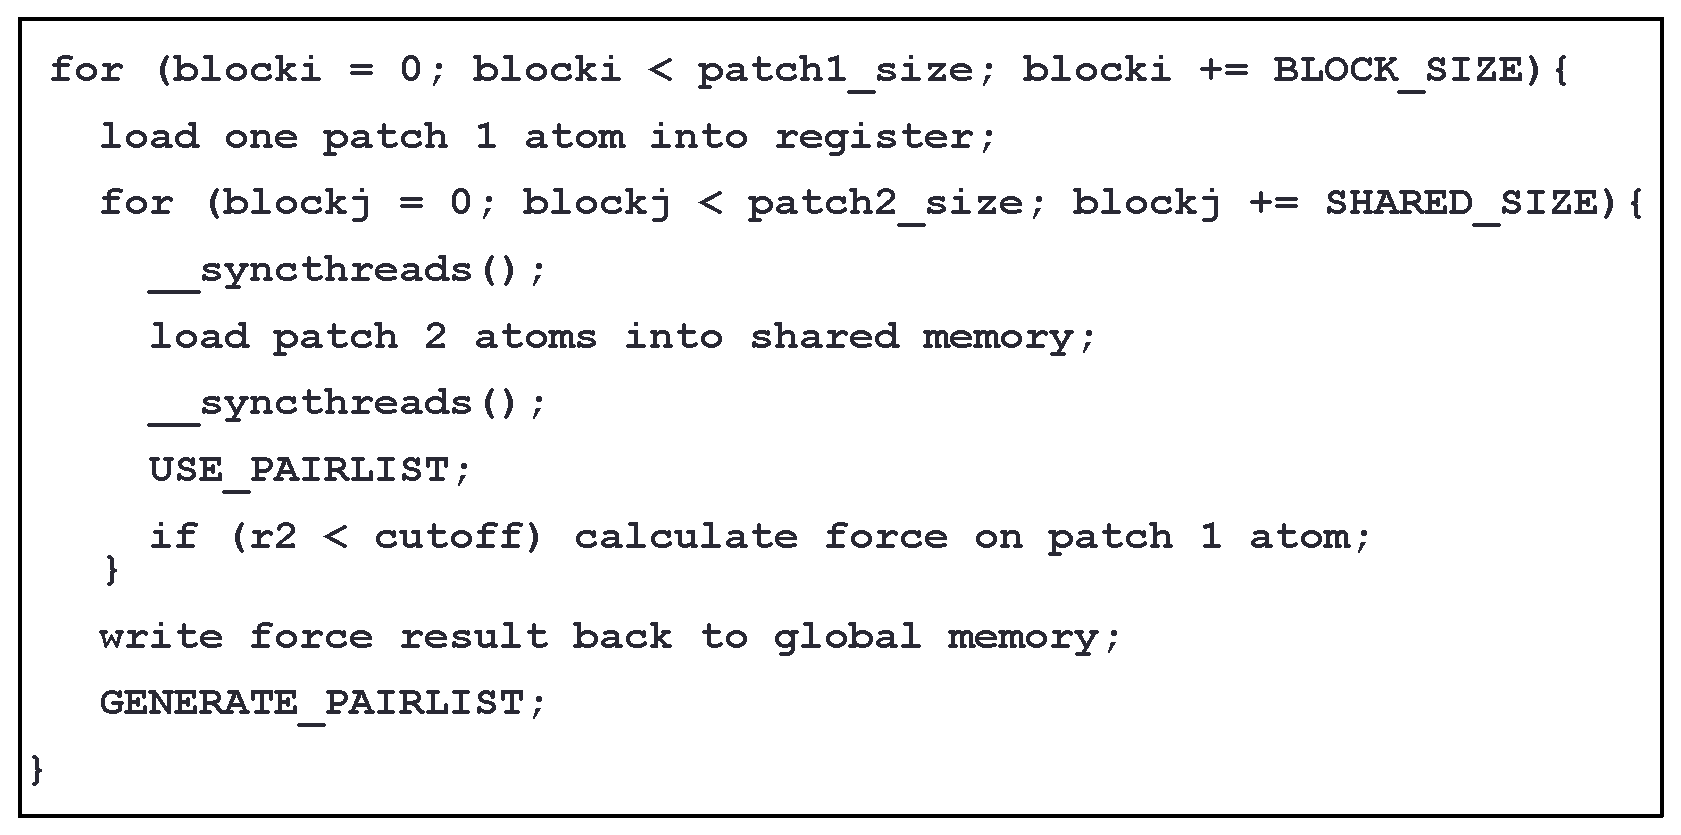
\includegraphics[width=4.0in]{figs/pseudocode.eps}
\caption{Pseudocode for GPU kernel force calculation}
\label{figs:pseudocode}
%\vspace{-0.5cm}
\end{figure}

After profiling the performance of the GPU kernel, we acquired the following observations:
(1) force calculation dominates the most GPU time compared to data loads and stores;
(2) there are great control divergence among different threads due to thread synchronization, which means some threads take a really long time
to reach the synchronization where other threads reach it very quickly. However, all threads in the block have to wait for everyone to
reach the synchronization before they can process further. Besides, use of pairlist may aggravate the divergence.
Based on above observations, we proposed several optimization approaches to reduce the control
divergence. They are described in detail in following sections.

\subsection{Optimizations}
\subsubsection{Patch 1 Atoms Tiling}

As indicated in Fig.~\ref{figs:pseudocode}, in the outer loop, all atoms in patch 2 need to be iterated for each patch 1 atom,
and there will be thread synchonization in every loop. According to that fact, we first considered the optimization of patch 1 atoms tiling,
in which each thread loads mulitple atoms instead of only one from patch 1 in the outer loop. By doing this, total number of outer loops can be reduced.
Because we merge work on each thread, synchronization latency can be decreased as indicated in Fig.~\ref{figs:divergence}.
Furthermore, data reuse can be improved because patch 2 atoms can be used for multiple patch 1 atoms in each outer loop.

\begin{figure}[h]
\centering
\setlength{\abovecaptionskip}{-1pt}
\setlength{\belowcaptionskip}{-2pt}
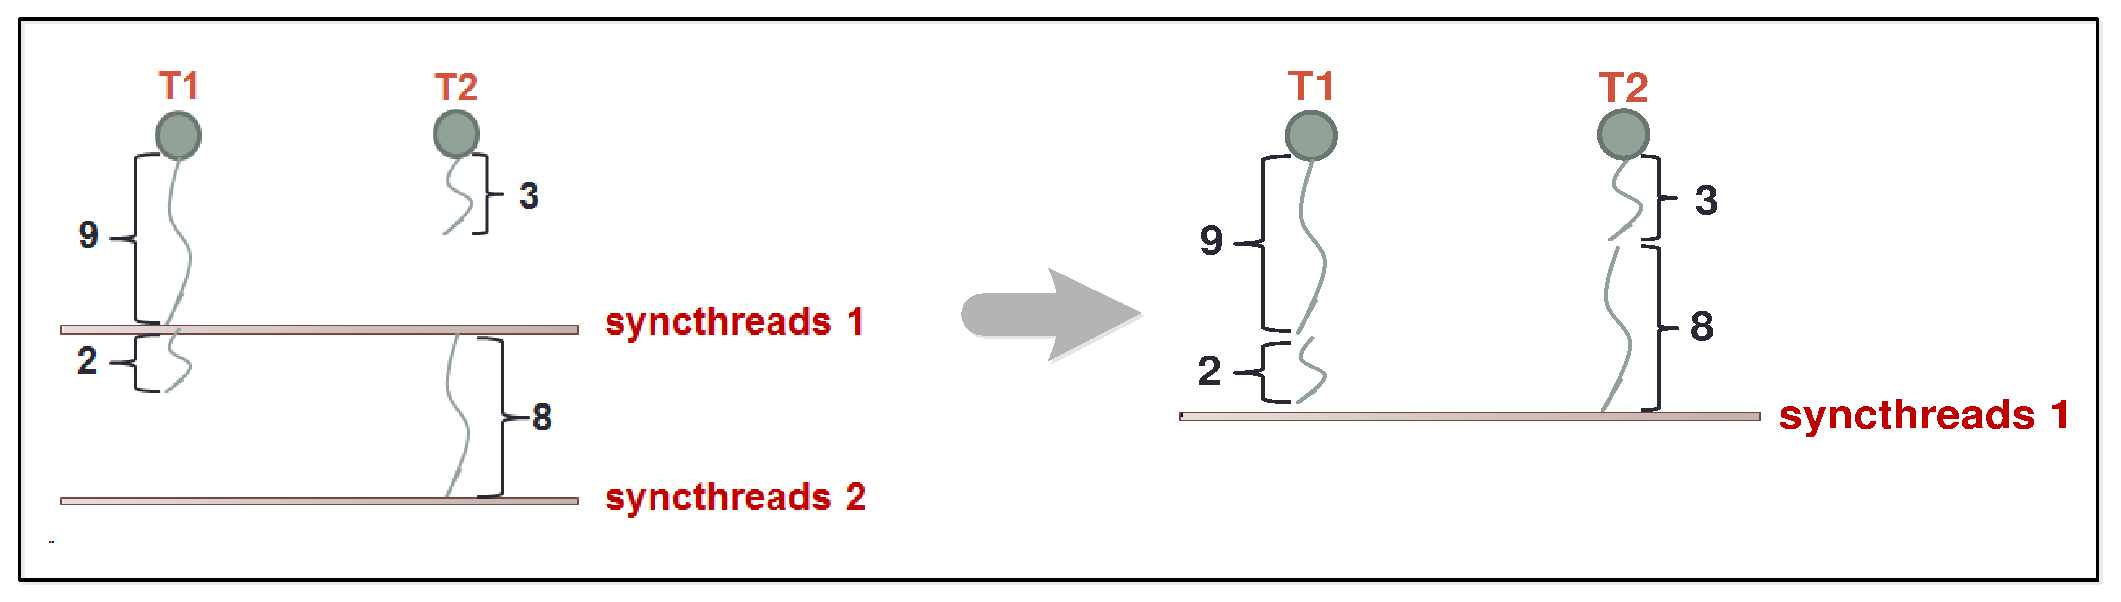
\includegraphics[width=6.0in]{figs/divergence.eps}
\caption{Reduce control divergence by patch 1 tiling}
\label{figs:divergence}
%\vspace{-0.5cm}
\end{figure}

\subsubsection{Patch 2 Atoms Tiling}
We also implemented tiling for loading patch 2 atoms to further reduce synchronization calls. In the original implementation in Fig.~\ref{figs:pseudocode},
for each inner loop, threads collaborate to load patch 2 atoms for one time. Instead, we make threads load multiple times in each inner loop to reduce the
total number of inner loops.

\begin{figure}[h]
\centering
\setlength{\abovecaptionskip}{-1pt}
\setlength{\belowcaptionskip}{-2pt}
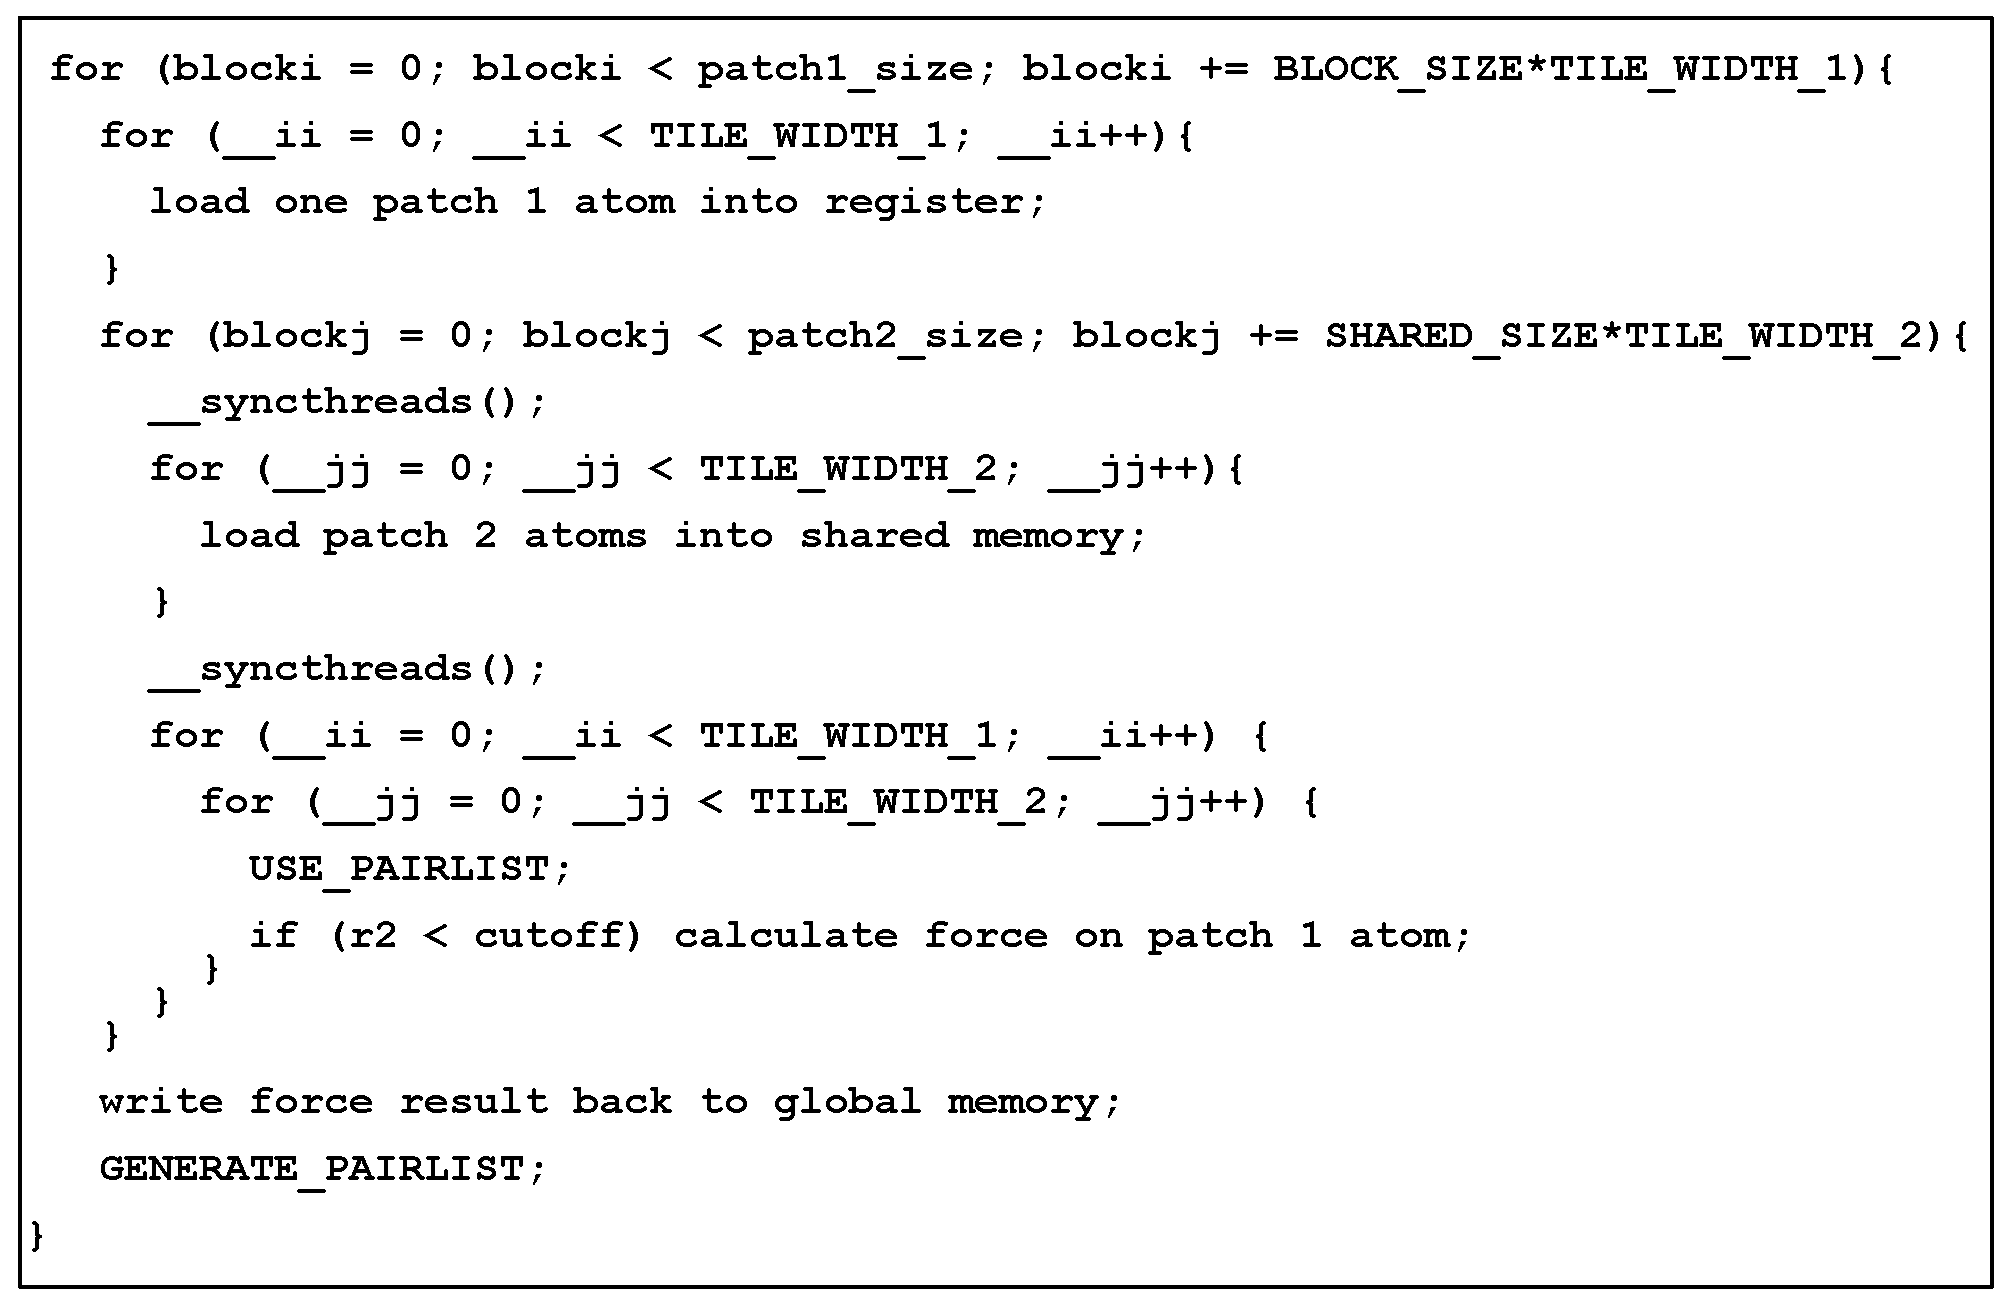
\includegraphics[width=4.0in]{figs/pseudocode-tile.eps}
\caption{Pseudocode for GPU kernel force calculation after tiling optimization}
\label{figs:pseudocode-tile}
%\vspace{-0.5cm}
\end{figure}

\subsubsection{Patch 1 Atoms Sorting}


\section{Performance Results}
  \textbf{Results on GPU and CPU load balance}: Fig.~\ref{figs:cpu-gpu-balance} 
  shows two time steps of the timeline of running DHFR using 4 CPU cores and 1 GPU. 
  In the first time step, all work is offload to GPU, which is the original design.
  The time cost for this step is $848 ms$. After applying the new balance scheme
  we discussed in section~\ref{sec:balance}, the time line is shown in the second step.
  We can see that all 4 CPU cores and the GPU is kept busy all the time. The time step 
  is $178 ms$, which is 4.8x speedup.
On Blue Waters, we achieved speedup of 1.3x due to the fast GPU.

\begin{figure}[h]
\centering
\includegraphics[width=6.5in]{figs/gpu-cpu-balance-timeline.png}
\caption{Timeline of running DHFR before and after load balance}
\label{figs:cpu-gpu-balance}
\end{figure}

\textbf{GPU kernel optimization results}: For tiling of patch 1 atoms, on the first
machine with GTX8800 GPU, we observed performance improvement as indicated in Fig.~\ref{figs:tile1-perf}.
The best performance improvement is 22\% when tile width is larger or equal to 4. Because the total
number of atoms in patch 1 is around 400, which takes 4 loops to be loaded and calculated on.
On JYC, we didn't see any improvement. With the help of profiling tools (``nvvp''), we found that after we increased tiling width for patch 1 atoms,
the amount of shared memory used by pairlist per thread is also rised. On this GPU, the occupancy is bounded by shared memory usage.
Therefore, increasing the total amount of shared memory usage leads to the decreasing of active thread blocks per SM.
As a result, the occupancy is reduced below 50\%, less than the original version.

However for GTX8800, the occupancy keeps the same for the cases of using tiling or not. This
is because its occupancy is bounded by register usage not shared memory usage, and we didn't change the number of registers per thread.
On the other hand, because GTX8800 is a quite old machine, the overhead of synchronization
divergence is more outstanding than JYC, therefore tiling of patch 1 atoms is able to improve its performance by reducing
synchronization latency.

\begin{figure}[h]
\centering
\setlength{\abovecaptionskip}{-1pt}
\setlength{\belowcaptionskip}{-2pt}
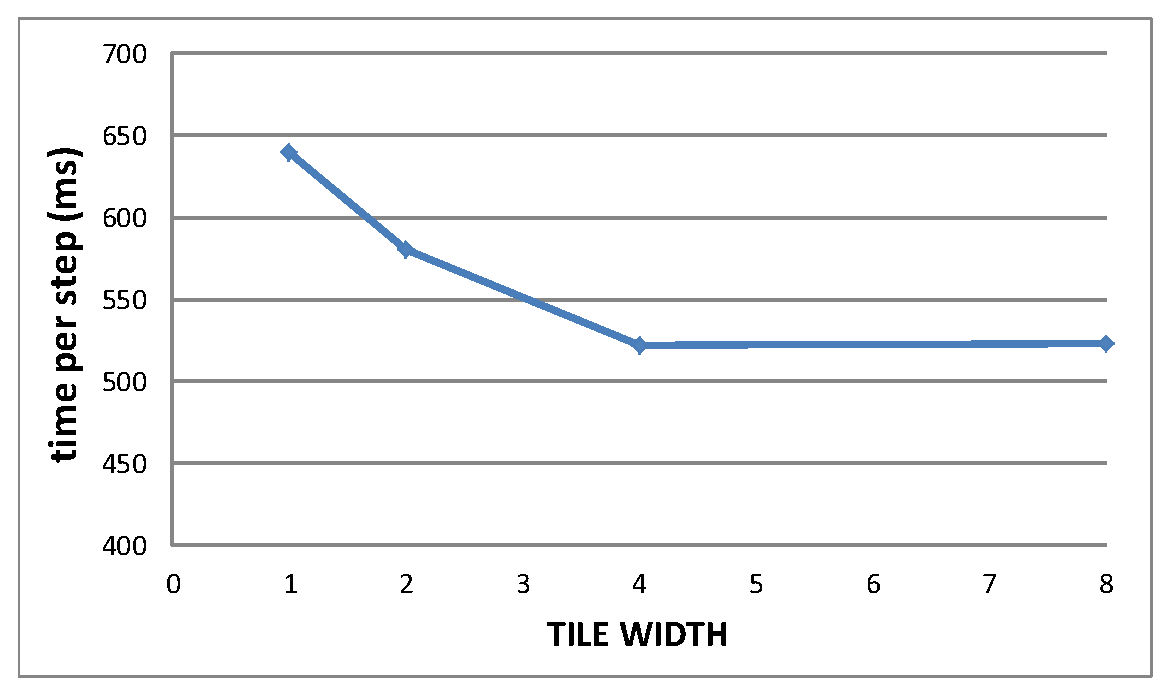
\includegraphics[width=4.0in]{figs/tile1-perf.eps}
\caption{Performance Improvement for tiling of patch 1 atoms}
\label{figs:tile1-perf}
%\vspace{-0.5cm}
\end{figure}

After implementing tiling of patch 2 atoms, we still didn't see performance improvement, because usage
of shared memory is continuing being increased and the occupancy is reduced. 

We also implemented the sorting strategy in the code, but didn't see any performance improvement. There are two
reasons for this: (1) after sorting, global memory access patterns for patch 1 atoms are not coalesced any more but become
very random, therefore overhead of load and store is increased. In other words, even though we make computation pattern regular
by sorting strategy, the memory access pattern becomes irregular. (2) Since we sort patch 1 atoms based on workload
on each atom, it makes sense when atoms in patch 2 are completely tiled. However, due to the shared memory
reason discussed above, tiling of patch 2 atoms makes performance worse, and it outweighs the benefit of sorting strategy.





\section{Conclusion and Discussion}
In this report, we have presented summary of our work on performance analysis and optimization for NAMD GPU implementation.
Our work is composed by two main aspects: one is GPU kernel optimization, and another is GPU / CPU load balancing. For both of them,
we tried different approaches to reduce divergence among threads and between GPU and CPUs. For GPU / CPU load balancing,
we first profiled the timeline when running program with 1 GPU with multiple CPUs and observed that nonbonded work on GPU is the bottleneck. Therefore
we offload part of nonbonded work from GPU to CPUs. For GPU kernel implemenation, we used CUDA profiling tools to get
GPU timing, occupancy, memory usage, etc, and observed that force calculation dominates most time. Based on our observation,
we proposed the tiling approach and sorting strategy to reduce control divergence caused by synchronization. We tested our code on two different machines to reflect
performance on different architecture configurations. 

In our future work, for load balancing, we plan to use more intelligent instrumentation-based balance scheme when assigning work to CPU and GPU.
For GPU kernel optimization, we plan to use a better strategy to sort atoms in the patch so that works on different threads can be assigned in a more even way.


\bibliographystyle{abbrv}
\bibliography{group,cited}
\end{document}


